\chapter{User interface design}
The following are simple mockups of how the \mts{} app should appear. In the case of the webapp, the required design is very much the same.

First, is a general overview of how the different screens are navigated by the user.

\begin{center}
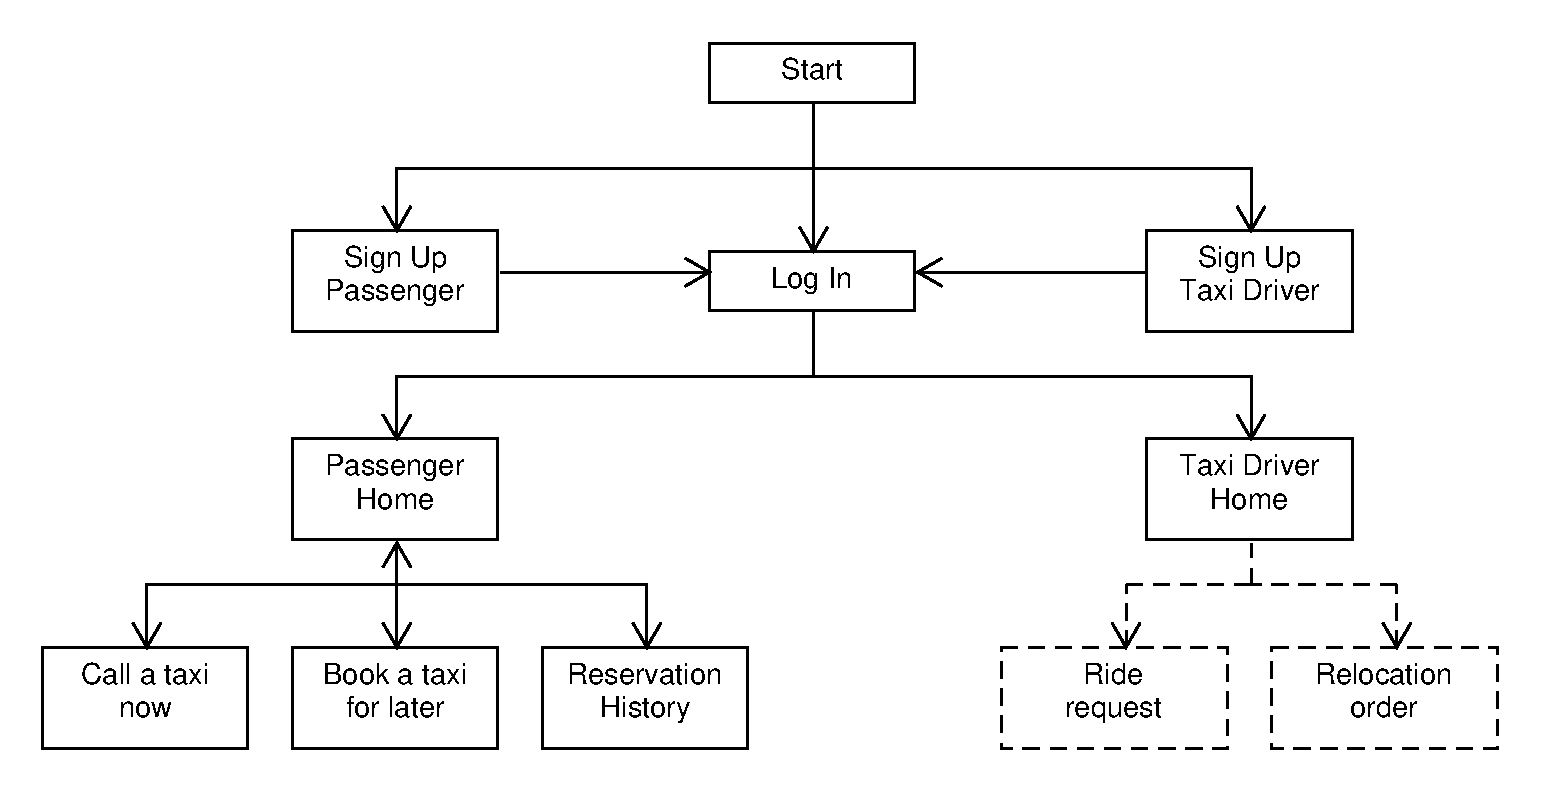
\includegraphics[width=\textwidth]{tex-images/ui-general}
\end{center}

In the following pages, several mockups of the main screens.


\begin{figure}
\centering
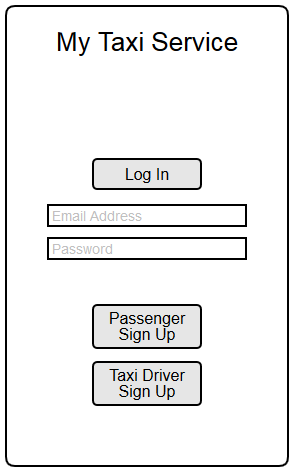
\includegraphics{tex-images/ui-app}
\caption{Sign Up / Log in view}
\end{figure}



\begin{figure}
\centering
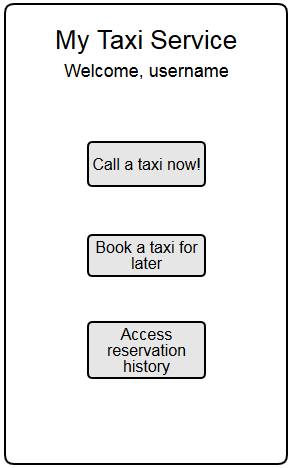
\includegraphics{tex-images/ui-passenger-home}
\caption{Passenger home}
\end{figure}

\begin{figure}
\centering
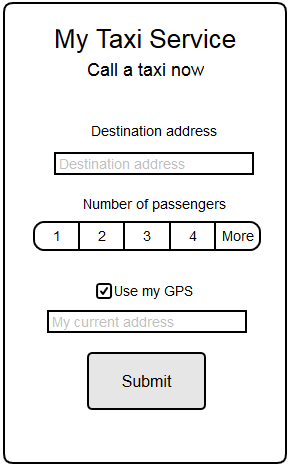
\includegraphics{tex-images/ui-passenger-call-taxi-now}
\caption{Call a taxi now function view}
\end{figure}

\begin{figure}
\centering
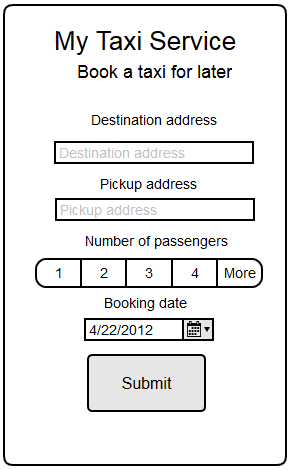
\includegraphics{tex-images/ui-passenger-book}
\caption{Booking function view}
\end{figure}

\begin{figure}
\centering
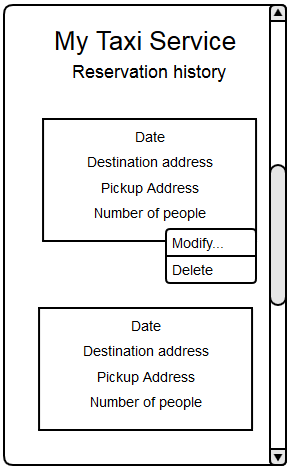
\includegraphics{tex-images/ui-passenger-history}
\caption{Reservation history view}
\end{figure}



\begin{figure}
\centering
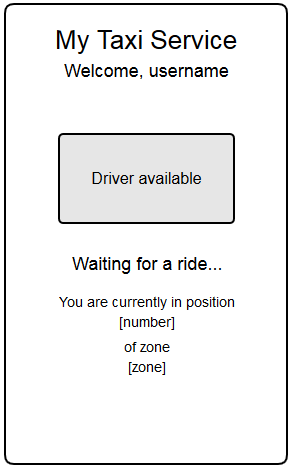
\includegraphics{tex-images/ui-driver-home}
\caption{Taxi driver home}
\end{figure}

\begin{figure}
\centering
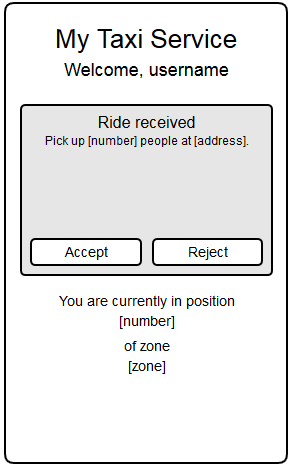
\includegraphics{tex-images/ui-driver-ride}
\caption{Taxi driver receives a ride request}
\end{figure}

\begin{figure}
\centering
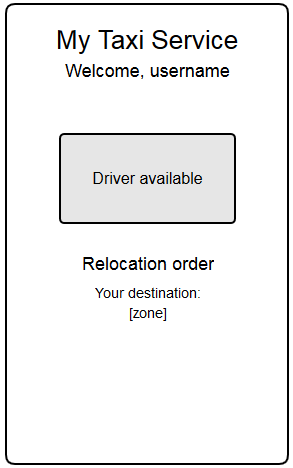
\includegraphics{tex-images/ui-driver-relocation}
\caption{Taxi driver receives a relocation request}
\end{figure}

\cleardoublepage